\section{The half-infinite double chain}

For the half-infinite double we define the Hamiltonian as
\begin{equation}
  \label{eq:1}
  H = \sum_{i = 1}^{\infty}\epsilon\left[\ket{i,1}\bra{i,1}+\ket{i,2}\bra{i,2}\right]+\left[\ket{i, 1}\bra{i+1,
      1}+\ket{i,2}\bra{i+1, 2}\right]+t\left[\ket{i,1}\bra{i,2}+h.c.\right].
\end{equation}
\todo{is h.c. correctly set?}
However in this model one assumes, that the binding $t$ is the same
between the positions parallel to the chain and between the upper and
lower site of position $i$ in the chain.
A more general approach would be to also take models into account
where the binding $t$ and $\overline{t}$ aren't the same as it is
depicted in figure~\ref{fig:half-inf-double-chain}.

\begin{figure}[hbt!]
  \centering
  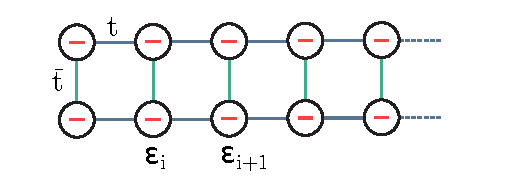
\includegraphics{pics/double_chain_different_t.pdf}
  \caption{Half-infinite double chain}
  \label{fig:half-inf-double-chain}
\end{figure}

For this one needs to just slightly alter the Hamiltonian of equation~\ref{eq:1} to
\begin{equation}
  \label{eq:2}
  H = \sum_{i = 1}^{\infty}\epsilon\left[\ket{i,1}\bra{i,1}+\ket{i,2}\bra{i,2}\right]+t\left[\ket{i, 1}\bra{i+1,
      1}+\ket{i,2}\bra{i+1, 2}+h.c.\right]+\overline{t}\left[\ket{i,1}\bra{i,2}+h.c.\right].
\end{equation}
%%% Local Variables:
%%% mode: latex
%%% TeX-master: "../MainDocument"
%%% End:
